% Options for packages loaded elsewhere
\PassOptionsToPackage{unicode}{hyperref}
\PassOptionsToPackage{hyphens}{url}
\PassOptionsToPackage{dvipsnames,svgnames,x11names}{xcolor}
%
\documentclass[
  letterpaper,
  DIV=11,
  numbers=noendperiod]{scrartcl}

\usepackage{amsmath,amssymb}
\usepackage{lmodern}
\usepackage{iftex}
\ifPDFTeX
  \usepackage[T1]{fontenc}
  \usepackage[utf8]{inputenc}
  \usepackage{textcomp} % provide euro and other symbols
\else % if luatex or xetex
  \usepackage{unicode-math}
  \defaultfontfeatures{Scale=MatchLowercase}
  \defaultfontfeatures[\rmfamily]{Ligatures=TeX,Scale=1}
\fi
% Use upquote if available, for straight quotes in verbatim environments
\IfFileExists{upquote.sty}{\usepackage{upquote}}{}
\IfFileExists{microtype.sty}{% use microtype if available
  \usepackage[]{microtype}
  \UseMicrotypeSet[protrusion]{basicmath} % disable protrusion for tt fonts
}{}
\makeatletter
\@ifundefined{KOMAClassName}{% if non-KOMA class
  \IfFileExists{parskip.sty}{%
    \usepackage{parskip}
  }{% else
    \setlength{\parindent}{0pt}
    \setlength{\parskip}{6pt plus 2pt minus 1pt}}
}{% if KOMA class
  \KOMAoptions{parskip=half}}
\makeatother
\usepackage{xcolor}
\setlength{\emergencystretch}{3em} % prevent overfull lines
\setcounter{secnumdepth}{-\maxdimen} % remove section numbering
% Make \paragraph and \subparagraph free-standing
\ifx\paragraph\undefined\else
  \let\oldparagraph\paragraph
  \renewcommand{\paragraph}[1]{\oldparagraph{#1}\mbox{}}
\fi
\ifx\subparagraph\undefined\else
  \let\oldsubparagraph\subparagraph
  \renewcommand{\subparagraph}[1]{\oldsubparagraph{#1}\mbox{}}
\fi


\providecommand{\tightlist}{%
  \setlength{\itemsep}{0pt}\setlength{\parskip}{0pt}}\usepackage{longtable,booktabs,array}
\usepackage{calc} % for calculating minipage widths
% Correct order of tables after \paragraph or \subparagraph
\usepackage{etoolbox}
\makeatletter
\patchcmd\longtable{\par}{\if@noskipsec\mbox{}\fi\par}{}{}
\makeatother
% Allow footnotes in longtable head/foot
\IfFileExists{footnotehyper.sty}{\usepackage{footnotehyper}}{\usepackage{footnote}}
\makesavenoteenv{longtable}
\usepackage{graphicx}
\makeatletter
\def\maxwidth{\ifdim\Gin@nat@width>\linewidth\linewidth\else\Gin@nat@width\fi}
\def\maxheight{\ifdim\Gin@nat@height>\textheight\textheight\else\Gin@nat@height\fi}
\makeatother
% Scale images if necessary, so that they will not overflow the page
% margins by default, and it is still possible to overwrite the defaults
% using explicit options in \includegraphics[width, height, ...]{}
\setkeys{Gin}{width=\maxwidth,height=\maxheight,keepaspectratio}
% Set default figure placement to htbp
\makeatletter
\def\fps@figure{htbp}
\makeatother
\newlength{\cslhangindent}
\setlength{\cslhangindent}{1.5em}
\newlength{\csllabelwidth}
\setlength{\csllabelwidth}{3em}
\newlength{\cslentryspacingunit} % times entry-spacing
\setlength{\cslentryspacingunit}{\parskip}
\newenvironment{CSLReferences}[2] % #1 hanging-ident, #2 entry spacing
 {% don't indent paragraphs
  \setlength{\parindent}{0pt}
  % turn on hanging indent if param 1 is 1
  \ifodd #1
  \let\oldpar\par
  \def\par{\hangindent=\cslhangindent\oldpar}
  \fi
  % set entry spacing
  \setlength{\parskip}{#2\cslentryspacingunit}
 }%
 {}
\usepackage{calc}
\newcommand{\CSLBlock}[1]{#1\hfill\break}
\newcommand{\CSLLeftMargin}[1]{\parbox[t]{\csllabelwidth}{#1}}
\newcommand{\CSLRightInline}[1]{\parbox[t]{\linewidth - \csllabelwidth}{#1}\break}
\newcommand{\CSLIndent}[1]{\hspace{\cslhangindent}#1}

\KOMAoption{captions}{tableheading}
\makeatletter
\makeatother
\makeatletter
\makeatother
\makeatletter
\@ifpackageloaded{caption}{}{\usepackage{caption}}
\AtBeginDocument{%
\ifdefined\contentsname
  \renewcommand*\contentsname{Table of contents}
\else
  \newcommand\contentsname{Table of contents}
\fi
\ifdefined\listfigurename
  \renewcommand*\listfigurename{List of Figures}
\else
  \newcommand\listfigurename{List of Figures}
\fi
\ifdefined\listtablename
  \renewcommand*\listtablename{List of Tables}
\else
  \newcommand\listtablename{List of Tables}
\fi
\ifdefined\figurename
  \renewcommand*\figurename{Figure}
\else
  \newcommand\figurename{Figure}
\fi
\ifdefined\tablename
  \renewcommand*\tablename{Table}
\else
  \newcommand\tablename{Table}
\fi
}
\@ifpackageloaded{float}{}{\usepackage{float}}
\floatstyle{ruled}
\@ifundefined{c@chapter}{\newfloat{codelisting}{h}{lop}}{\newfloat{codelisting}{h}{lop}[chapter]}
\floatname{codelisting}{Listing}
\newcommand*\listoflistings{\listof{codelisting}{List of Listings}}
\makeatother
\makeatletter
\@ifpackageloaded{caption}{}{\usepackage{caption}}
\@ifpackageloaded{subcaption}{}{\usepackage{subcaption}}
\makeatother
\makeatletter
\@ifpackageloaded{tcolorbox}{}{\usepackage[many]{tcolorbox}}
\makeatother
\makeatletter
\@ifundefined{shadecolor}{\definecolor{shadecolor}{rgb}{.97, .97, .97}}
\makeatother
\makeatletter
\makeatother
\ifLuaTeX
  \usepackage{selnolig}  % disable illegal ligatures
\fi
\IfFileExists{bookmark.sty}{\usepackage{bookmark}}{\usepackage{hyperref}}
\IfFileExists{xurl.sty}{\usepackage{xurl}}{} % add URL line breaks if available
\urlstyle{same} % disable monospaced font for URLs
\hypersetup{
  pdftitle={Modelling a vaccination campaign against monkeypox in Mexico},
  pdfauthor={Rodrigo Zepeda-Tello},
  colorlinks=true,
  linkcolor={blue},
  filecolor={Maroon},
  citecolor={Blue},
  urlcolor={Blue},
  pdfcreator={LaTeX via pandoc}}

\title{Modelling a vaccination campaign against monkeypox in Mexico}
\author{Rodrigo Zepeda-Tello}
\date{}

\begin{document}
\maketitle
\ifdefined\Shaded\renewenvironment{Shaded}{\begin{tcolorbox}[enhanced, interior hidden, boxrule=0pt, breakable, borderline west={3pt}{0pt}{shadecolor}, sharp corners, frame hidden]}{\end{tcolorbox}}\fi

\hypertarget{introduction}{%
\subsection{Introduction}\label{introduction}}

\hypertarget{data}{%
\subsection{Data}\label{data}}

\hypertarget{monkeypox-cases}{%
\subsubsection{Monkeypox cases}\label{monkeypox-cases}}

Weekly incident cases were obtained from the reports of the General
Directorate of Epidemiology of Mexico (Secretaría de Salud 2022).

\hypertarget{parameter-information}{%
\subsubsection{Parameter information}\label{parameter-information}}

\hypertarget{model}{%
\subsection{Model}\label{model}}

Our model is a pair-formation Susceptible-Exposed-Infected-Recovered
(SEIR) system of differential equations adapted from
\href{https://doi.org/10.1101/2022.08.17.22278897}{Betti, Farrell, and
Heffernan (2022)}. Briefly, in pair formation models the infection is
driven by the rate of \textbf{partnership} formation between individuals
and transmission probabilities per sexual act within the partnership
\href{https://doi.org/10.1016/j.idm.2017.07.002}{Kretzschmar and Heijne
(2017)}. In these models, \textbf{single} individuals (individuals that
don't form partnerships) don't get infected nor infect others.
Individuals within \textbf{partnerships} only get infected with a
probability \(\phi\) if the other individual within that partnership is
infected already.

\begin{figure}

{\centering 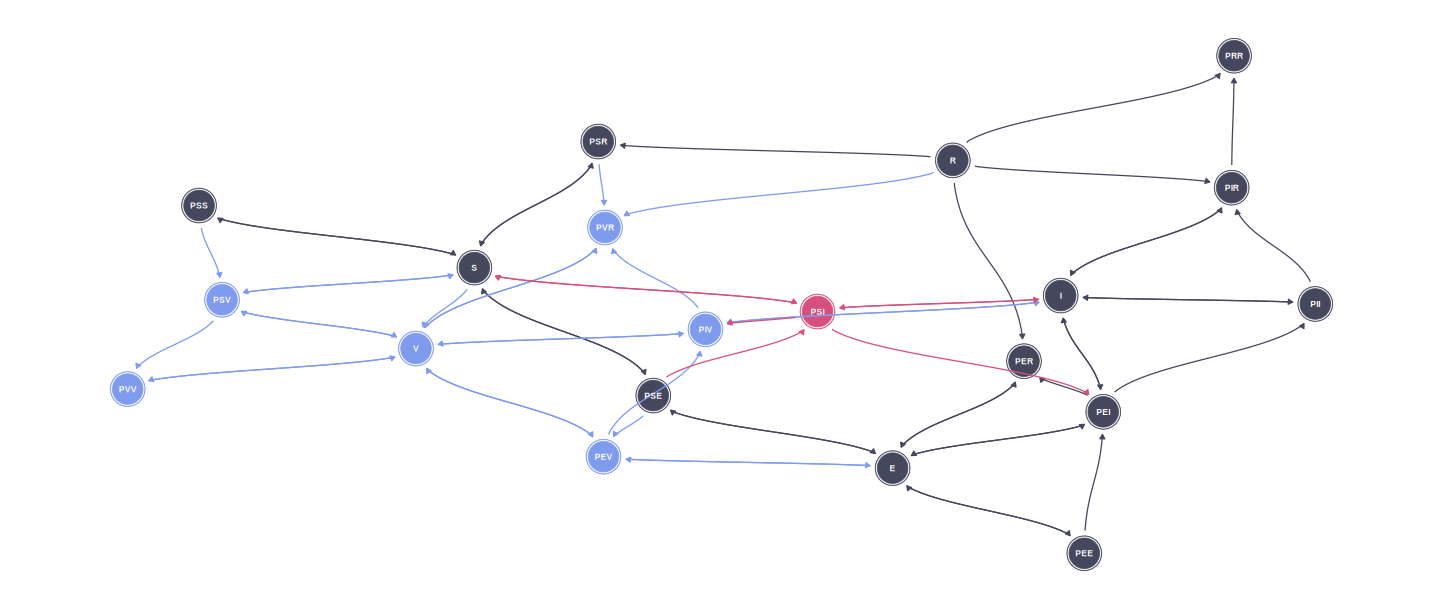
\includegraphics[width=1\textwidth,height=\textheight]{images/model_diagram.svg}

}

\caption{\label{fig-diagram-model}Diagram of the model. Bright red node
\(P_{SI}\) is the main driver of the infection as it represents a
partnership between a Susceptible and an Infected individual. This
partnership irradiates the infection towards \(P_{EI}\) if the
susceptible becomes infected and the partnership continues. The
partnership might also dissolve into the susceptible \(S\) and the
infected \(I\) or might not result in an infection but a recovery of the
infected partner \(P_{SR}\).}

\end{figure}

The variables of the model are specified in Table~\ref{tbl-variables}.

\hypertarget{tbl-variables}{}
\begin{longtable}[]{@{}
  >{\raggedright\arraybackslash}p{(\columnwidth - 2\tabcolsep) * \real{0.2500}}
  >{\raggedright\arraybackslash}p{(\columnwidth - 2\tabcolsep) * \real{0.7500}}@{}}
\caption{\label{tbl-variables}Variables used in the model
Equation~\ref{eq-model}.}\tabularnewline
\toprule()
\begin{minipage}[b]{\linewidth}\raggedright
Variable
\end{minipage} & \begin{minipage}[b]{\linewidth}\raggedright
Definition
\end{minipage} \\
\midrule()
\endfirsthead
\toprule()
\begin{minipage}[b]{\linewidth}\raggedright
Variable
\end{minipage} & \begin{minipage}[b]{\linewidth}\raggedright
Definition
\end{minipage} \\
\midrule()
\endhead
\(S\) & \textbf{Single} susceptible individuals \\
\(E\) & \textbf{Single} exposed individuals \\
\(I\) & \textbf{Single} infected individuals \\
\(R\) & \textbf{Single} recovered individuals \\
\(V\) & \textbf{Single} vaccinated individuals \\
\(P_{kl}\) & \textbf{Partnership} of two individuals in which one
partner belongs to category \(k\) and the other to category \(l\)
(\emph{e.g.} \(P_{SI}\) represents a partnership between a susceptible
\(S\) and an infected \(I\) individual). \\
\bottomrule()
\end{longtable}

The differential equations representation for the model is:
\begin{equation}\protect\hypertarget{eq-model}{}{
\begin{align}
\frac{dS}{dt}      &= -(\rho + \nu) S + \sigma (2 P_{SS} + P_{SE} + P_{SI} + P_{SR} + P_{SV})\\
\frac{dE}{dt}      &= -(\rho + \theta) E + \sigma (P_{SE} + 2 P_{EE} + P_{EI} + P_{ER} + P_{EV})\\
\frac{dI}{dt}      &= -(\rho + \delta) I + \theta E + \sigma (P_{SI} + P_{EI} + 2P_{II} + P_{IR} + P_{IV})  \\
\frac{dR}{dt}      &= - \rho R + \delta I + \sigma (P_{SR} + P_{ER} + P_{IR} + 2 P_{RR} + P_{RV})  \\
\frac{dV}{dt}      &= - \rho V + \nu S  + \sigma (P_{SV} + P_{EV} + P_{IV} + P_{RV} + 2 P_{VV})  \\
\frac{dP_{SS}}{dt} &= \frac{1}{2}\rho \frac{S^2}{N} - (\sigma + 2 \nu) P_{SS} \\
\frac{dP_{SE}}{dt} &= \rho \frac{SE}{N} - (\sigma + \theta + \nu) P_{SE} \\
\frac{dP_{SI}}{dt} &= \rho (1 - h) \frac{SI}{N} + \theta P_{SE} - (\sigma + \phi h + \delta + \nu) P_{SI} \\
\frac{dP_{SR}}{dt} &= \rho \frac{SR}{N} + \delta P_{SI} - (\sigma  + \nu) P_{SR} \\
\frac{dP_{SV}}{dt} &= \rho \frac{SV}{N} + 2 \nu P_{SS} - (\sigma  + \nu) P_{SV} \\
\frac{dP_{EE}}{dt} &= \frac{1}{2} \rho \frac{E^2}{N} - (\sigma + 2 \theta) P_{EE} \\
\frac{dP_{EI}}{dt} &= \rho \frac{EI}{N} + \rho h \frac{SI}{N}  + \phi h P_{SI} + 2  \theta P_{EE} - (\sigma + \theta + \delta) P_{EI} \\
\frac{dP_{ER}}{dt} &= \rho \frac{ER}{N} + \delta P_{EI} - (\sigma + \theta) P_{ER} \\
\frac{dP_{EV}}{dt} &= \rho \frac{EV}{N} + \nu P_{SE} - (\sigma + \theta) P_{EV} \\
\frac{dP_{II}}{dt} &= \frac{1}{2} \rho \frac{I^2}{N} + \theta P_{EI} - (\sigma + 2 \delta) P_{II} \\
\frac{dP_{IR}}{dt} &= \rho \frac{IR}{N} + 2 \delta P_{II} + \theta P_{ER} - (\sigma + \delta) P_{IR} \\
\frac{dP_{IV}}{dt} &= \rho \frac{IV}{N} + \theta P_{EV} + \nu P_{SI} - (\sigma + \delta) P_{IV} \\
\frac{dP_{RR}}{dt} &= \frac{1}{2} \rho \frac{R^2}{N} + \delta P_{IR} - \sigma P_{RR} \\
\frac{dP_{RV}}{dt} &= \rho \frac{RV}{N} + \delta P_{IV} + \nu P_{SR} - \sigma P_{RV} \\
\frac{dP_{VV}}{dt} &= \frac{1}{2} \rho \frac{V^2}{N} + \nu P_{SV}  - \sigma  P_{VV} \\
\end{align}
}\label{eq-model}\end{equation}

With the parameters and their meanings are established in
Table~\ref{tbl-parameters}. As the model was fitted using a Bayesian
framework, \emph{prior} distributions for the parameters are also
specified in Table~\ref{tbl-parameters}.

\hypertarget{tbl-parameters}{}
\begin{longtable}[]{@{}ll@{}}
\caption{\label{tbl-parameters}Parameters used in the model
Equation~\ref{eq-model}.}\tabularnewline
\toprule()
Parameter & Definition \\
\midrule()
\endfirsthead
\toprule()
Parameter & Definition \\
\midrule()
\endhead
\(\rho\) & Partnership formation rate \\
\(\sigma\) & Partnership dissolution rate \\
\(\nu\) & Vaccination rate \\
\(\theta\) & Incubation rate \\
\(\delta\) & Infection recovery rate \\
\(h\) & Probability of transmission per contact \\
\(\phi\) & Contact rate per partnership \\
\bottomrule()
\end{longtable}

\hypertarget{code-availability}{%
\subsection{Code availability}\label{code-availability}}

Both the code and the data can be found in our
\href{https://github.com/rodrigoZepeda/mpx}{Github repository}

\hypertarget{references}{%
\subsection*{References}\label{references}}
\addcontentsline{toc}{subsection}{References}

\hypertarget{refs}{}
\begin{CSLReferences}{1}{0}
\leavevmode\vadjust pre{\hypertarget{ref-betti2022pair}{}}%
Betti, Matthew, Lauren Farrell, and Jane M Heffernan. 2022. {``A Pair
Formation Model with Recovery: Application to Monkeypox.''}
\emph{medRxiv}.

\leavevmode\vadjust pre{\hypertarget{ref-kretzschmar2017pair}{}}%
Kretzschmar, Mirjam, and Janneke CM Heijne. 2017. {``Pair Formation
Models for Sexually Transmitted Infections: A Primer.''}
\emph{Infectious Disease Modelling} 2 (3): 368--78.

\leavevmode\vadjust pre{\hypertarget{ref-mpxdge}{}}%
Secretaría de Salud. 2022. {``Informes Semanales Con Información de
Viruela Símica En México.''} \emph{Secretaría de Salud}.
\url{https://www.gob.mx/salud/documentos/informes-semanales-para-la-vigilancia-epidemiologica-de-viruela-simica-en-mexico}.

\end{CSLReferences}



\end{document}
